\documentclass[border=10pt]{standalone}
\usepackage{tikz}
\usetikzlibrary{arrows.meta, positioning, calc}

\begin{document}
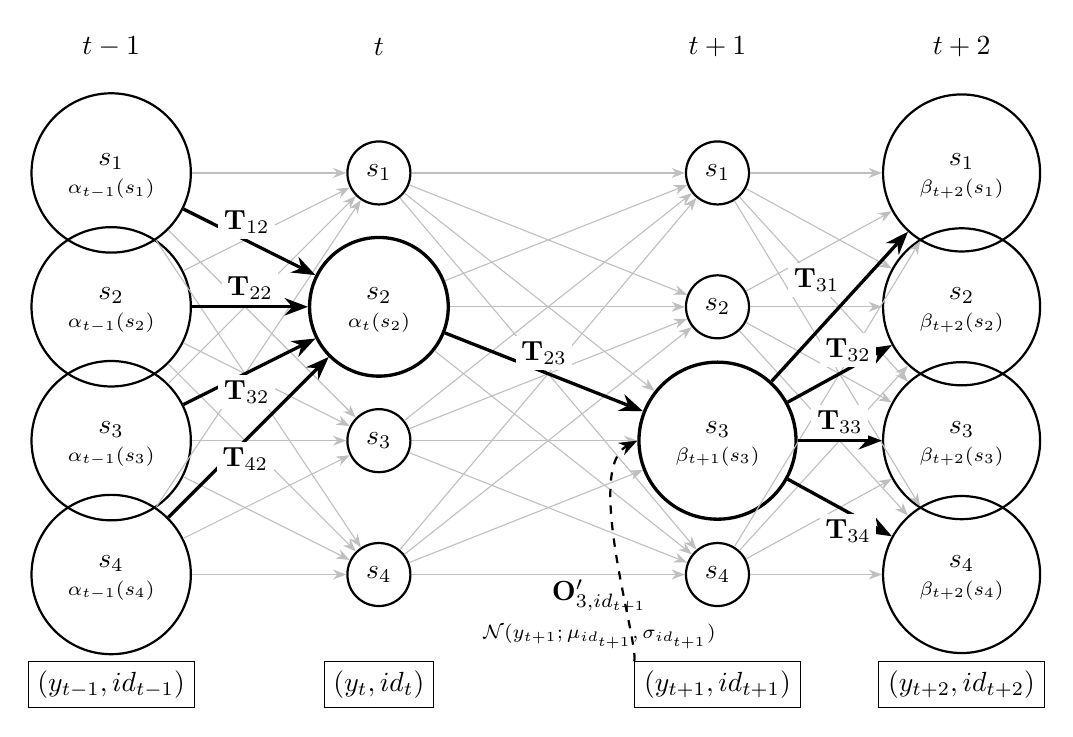
\begin{tikzpicture}[
    node distance=1.5cm and 2.5cm,
    state/.style={circle, draw, minimum size=0.8cm, thick},
    bigstate/.style={circle, draw, minimum size=1.35cm, thick},
    boldstate/.style={circle, draw, minimum size=1.35cm, very thick},
    arrow/.style={->, >=Stealth, gray!50, thin},
    boldarrow/.style={->, >=Stealth, black, very thick},
    dashedarrow/.style={->, >=Stealth, black, thick, dashed},
    translabel/.style={fill=white, inner sep=2pt}
]

% Time labels
\node at (0, 5.2) {$t-1$};
\node at (3.4, 5.2) {$t$};
\node at (7.7, 5.2) {$t+1$};
\node at (10.8, 5.2) {$t+2$};

% States at t-1
\node[bigstate] (s1t-1) at (0, 3.6) {\begin{tabular}{c}$s_1$\\[-2pt]\scriptsize$\alpha_{t-1}(s_1)$\end{tabular}};
\node[bigstate] (s2t-1) at (0, 1.9) {\begin{tabular}{c}$s_2$\\[-2pt]\scriptsize$\alpha_{t-1}(s_2)$\end{tabular}};
\node[bigstate] (s3t-1) at (0, 0.2) {\begin{tabular}{c}$s_3$\\[-2pt]\scriptsize$\alpha_{t-1}(s_3)$\end{tabular}};
\node[bigstate] (s4t-1) at (0, -1.5) {\begin{tabular}{c}$s_4$\\[-2pt]\scriptsize$\alpha_{t-1}(s_4)$\end{tabular}};

% States at t
\node[state] (s1t) at (3.4, 3.6) {$s_1$};
\node[boldstate] (s2t) at (3.4, 1.9) {\begin{tabular}{c}$s_2$\\[-2pt]\scriptsize$\alpha_t(s_2)$\end{tabular}};
\node[state] (s3t) at (3.4, 0.2) {$s_3$};
\node[state] (s4t) at (3.4, -1.5) {$s_4$};

% States at t+1
\node[state] (s1t+1) at (7.7, 3.6) {$s_1$};
\node[state] (s2t+1) at (7.7, 1.9) {$s_2$};
\node[boldstate] (s3t+1) at (7.7, 0.2) {\begin{tabular}{c}$s_3$\\[-2pt]\scriptsize$\beta_{t+1}(s_3)$\end{tabular}};
\node[state] (s4t+1) at (7.7, -1.5) {$s_4$};

% States at t+2
\node[bigstate] (s1t+2) at (10.8, 3.6) {\begin{tabular}{c}$s_1$\\[-2pt]\scriptsize$\beta_{t+2}(s_1)$\end{tabular}};
\node[bigstate] (s2t+2) at (10.8, 1.9) {\begin{tabular}{c}$s_2$\\[-2pt]\scriptsize$\beta_{t+2}(s_2)$\end{tabular}};
\node[bigstate] (s3t+2) at (10.8, 0.2) {\begin{tabular}{c}$s_3$\\[-2pt]\scriptsize$\beta_{t+2}(s_3)$\end{tabular}};
\node[bigstate] (s4t+2) at (10.8, -1.5) {\begin{tabular}{c}$s_4$\\[-2pt]\scriptsize$\beta_{t+2}(s_4)$\end{tabular}};

% All transitions (gray, thin) from t-1 to t
\foreach \i in {1,2,3,4} {
    \foreach \j in {1,2,3,4} {
        \draw[arrow] (s\i t-1) -- (s\j t);
    }
}

% All transitions (gray, thin) from t to t+1
\foreach \i in {1,2,3,4} {
    \foreach \j in {1,2,3,4} {
        \draw[arrow] (s\i t) -- (s\j t+1);
    }
}

% All transitions (gray, thin) from t+1 to t+2
\foreach \i in {1,2,3,4} {
    \foreach \j in {1,2,3,4} {
        \draw[arrow] (s\i t+1) -- (s\j t+2);
    }
}

% Bold transitions from t-1 to t
\draw[boldarrow] (s1t-1) -- (s2t) node[pos=0.48, above, translabel] {$\mathbf{T}_{12}$};
\draw[boldarrow] (s2t-1) -- (s2t) node[midway, above, translabel] {$\mathbf{T}_{22}$};
\draw[boldarrow] (s3t-1) -- (s2t) node[pos=0.48, below, translabel] {$\mathbf{T}_{32}$};
\draw[boldarrow] (s4t-1) -- (s2t) node[pos=0.48, below, translabel] {$\mathbf{T}_{42}$};

% Bold transitions from t to t+1
\draw[boldarrow] (s2t) -- (s3t+1) node[midway, above, translabel] {$\mathbf{T}_{23}$};

% Bold transitions from t+1 to t+2
\draw[boldarrow] (s3t+1) -- (s1t+2) node[pos=0.55, above left, translabel] {$\mathbf{T}_{31}$};
\draw[boldarrow] (s3t+1) -- (s2t+2) node[pos=0.58, above, translabel] {$\mathbf{T}_{32}$};
\draw[boldarrow] (s3t+1) -- (s3t+2) node[midway, above, translabel] {$\mathbf{T}_{33}$};
\draw[boldarrow] (s3t+1) -- (s4t+2) node[pos=0.58, below, translabel] {$\mathbf{T}_{34}$};

% Observation boxes
\node[draw, rectangle] (ot-1) at (0, -2.9) {$(y_{t-1}, id_{t-1})$};
\node[draw, rectangle] (ot) at (3.4, -2.9) {$(y_t, id_t)$};
\node[draw, rectangle] (ot+1) at (7.7, -2.9) {$(y_{t+1}, id_{t+1})$};
\node[draw, rectangle] (ot+2) at (10.8, -2.9) {$(y_{t+2}, id_{t+2})$};

% Observation model
\draw[dashedarrow] (ot+1.north west) .. controls (6.7, -2.35) and (6.0, -0.15) .. (s3t+1.west);
\node[align=center] at (6.2, -2.0) {$\mathbf{O}'_{3,id_{t+1}}$\\[2pt]\scriptsize$\mathcal{N}(y_{t+1}; \mu_{id_{t+1}}, \sigma_{id_{t+1}})$};

\end{tikzpicture}
\end{document}
